\chapter{Evaluation}

\section{Methodology}

As explained in Section \ref{subsec:selecting_dataset}, three sets of images were selected for research:

\begin{itemize}
    \item A full dataset containing all categories, with no class imbalance issues
    \item A dual dataset, with no class imbalance issues
    \item A `DMSO' dataset, which should show the most distinction between classes, but has class imbalance issues
\end{itemize}

Training and validating the autoencoder and regression models was done on the full dataset's 19,000 instances. We had 10,000 instances of this dataset left for testing, and 15,900 instances of the dual dataset, as well as 8,000 instances of the DMSO dataset. All datasets were consistently shuffled before training and testing with a random state parameter. Moreover, we had two versions of each dataset: one which has been noise-corrected, and one which has been background-corrected through the help of k-means colour segmentation. This dataset was denominated the `masked' dataset.

We are looking to evaluate the performance of our autoencoder and regression model on the unseen images of these datasets.

\begin{itemize}
    \item The success of the autoencoder model will be evaluated on its capacity at image reconstruction, as well as if the projection by t-SNE or UMAP of the images coded by the autoencoder show some underlying structure of the data.
    \item The regression model will be evaluated on how well it predicts interaction values for unseen images of immune cells.
\end{itemize}

\section{Autoencoder}

\subsection{How well can we reconstruct an image?}

%The task of an autoencoder is of the reconstruction of its input and how well the input is reconstructed. As such, we are looking to minimise the difference between the input to the model and its reconstruction. For a real-valued input, the difference would be calculated using the Mean-Squared-Error (MSE) loss, but because we are working in a normalised range of [0, 1], we are using the binary cross-entropy loss. The loss computed can then be considered as a probability of how close the two images are to each other. [should this be here or in implementation? repeated myself]

The following images show how the autoencoder performed on image reconstruction. [what to show: one image in each category + both masked and unmasked?]

\bigskip
\subsubsection{Full dataset}
\hfill
\hfill

\begin{figure}[h!]
    \centering
    \begin{subfigure}[h!]{0.45\textwidth}
        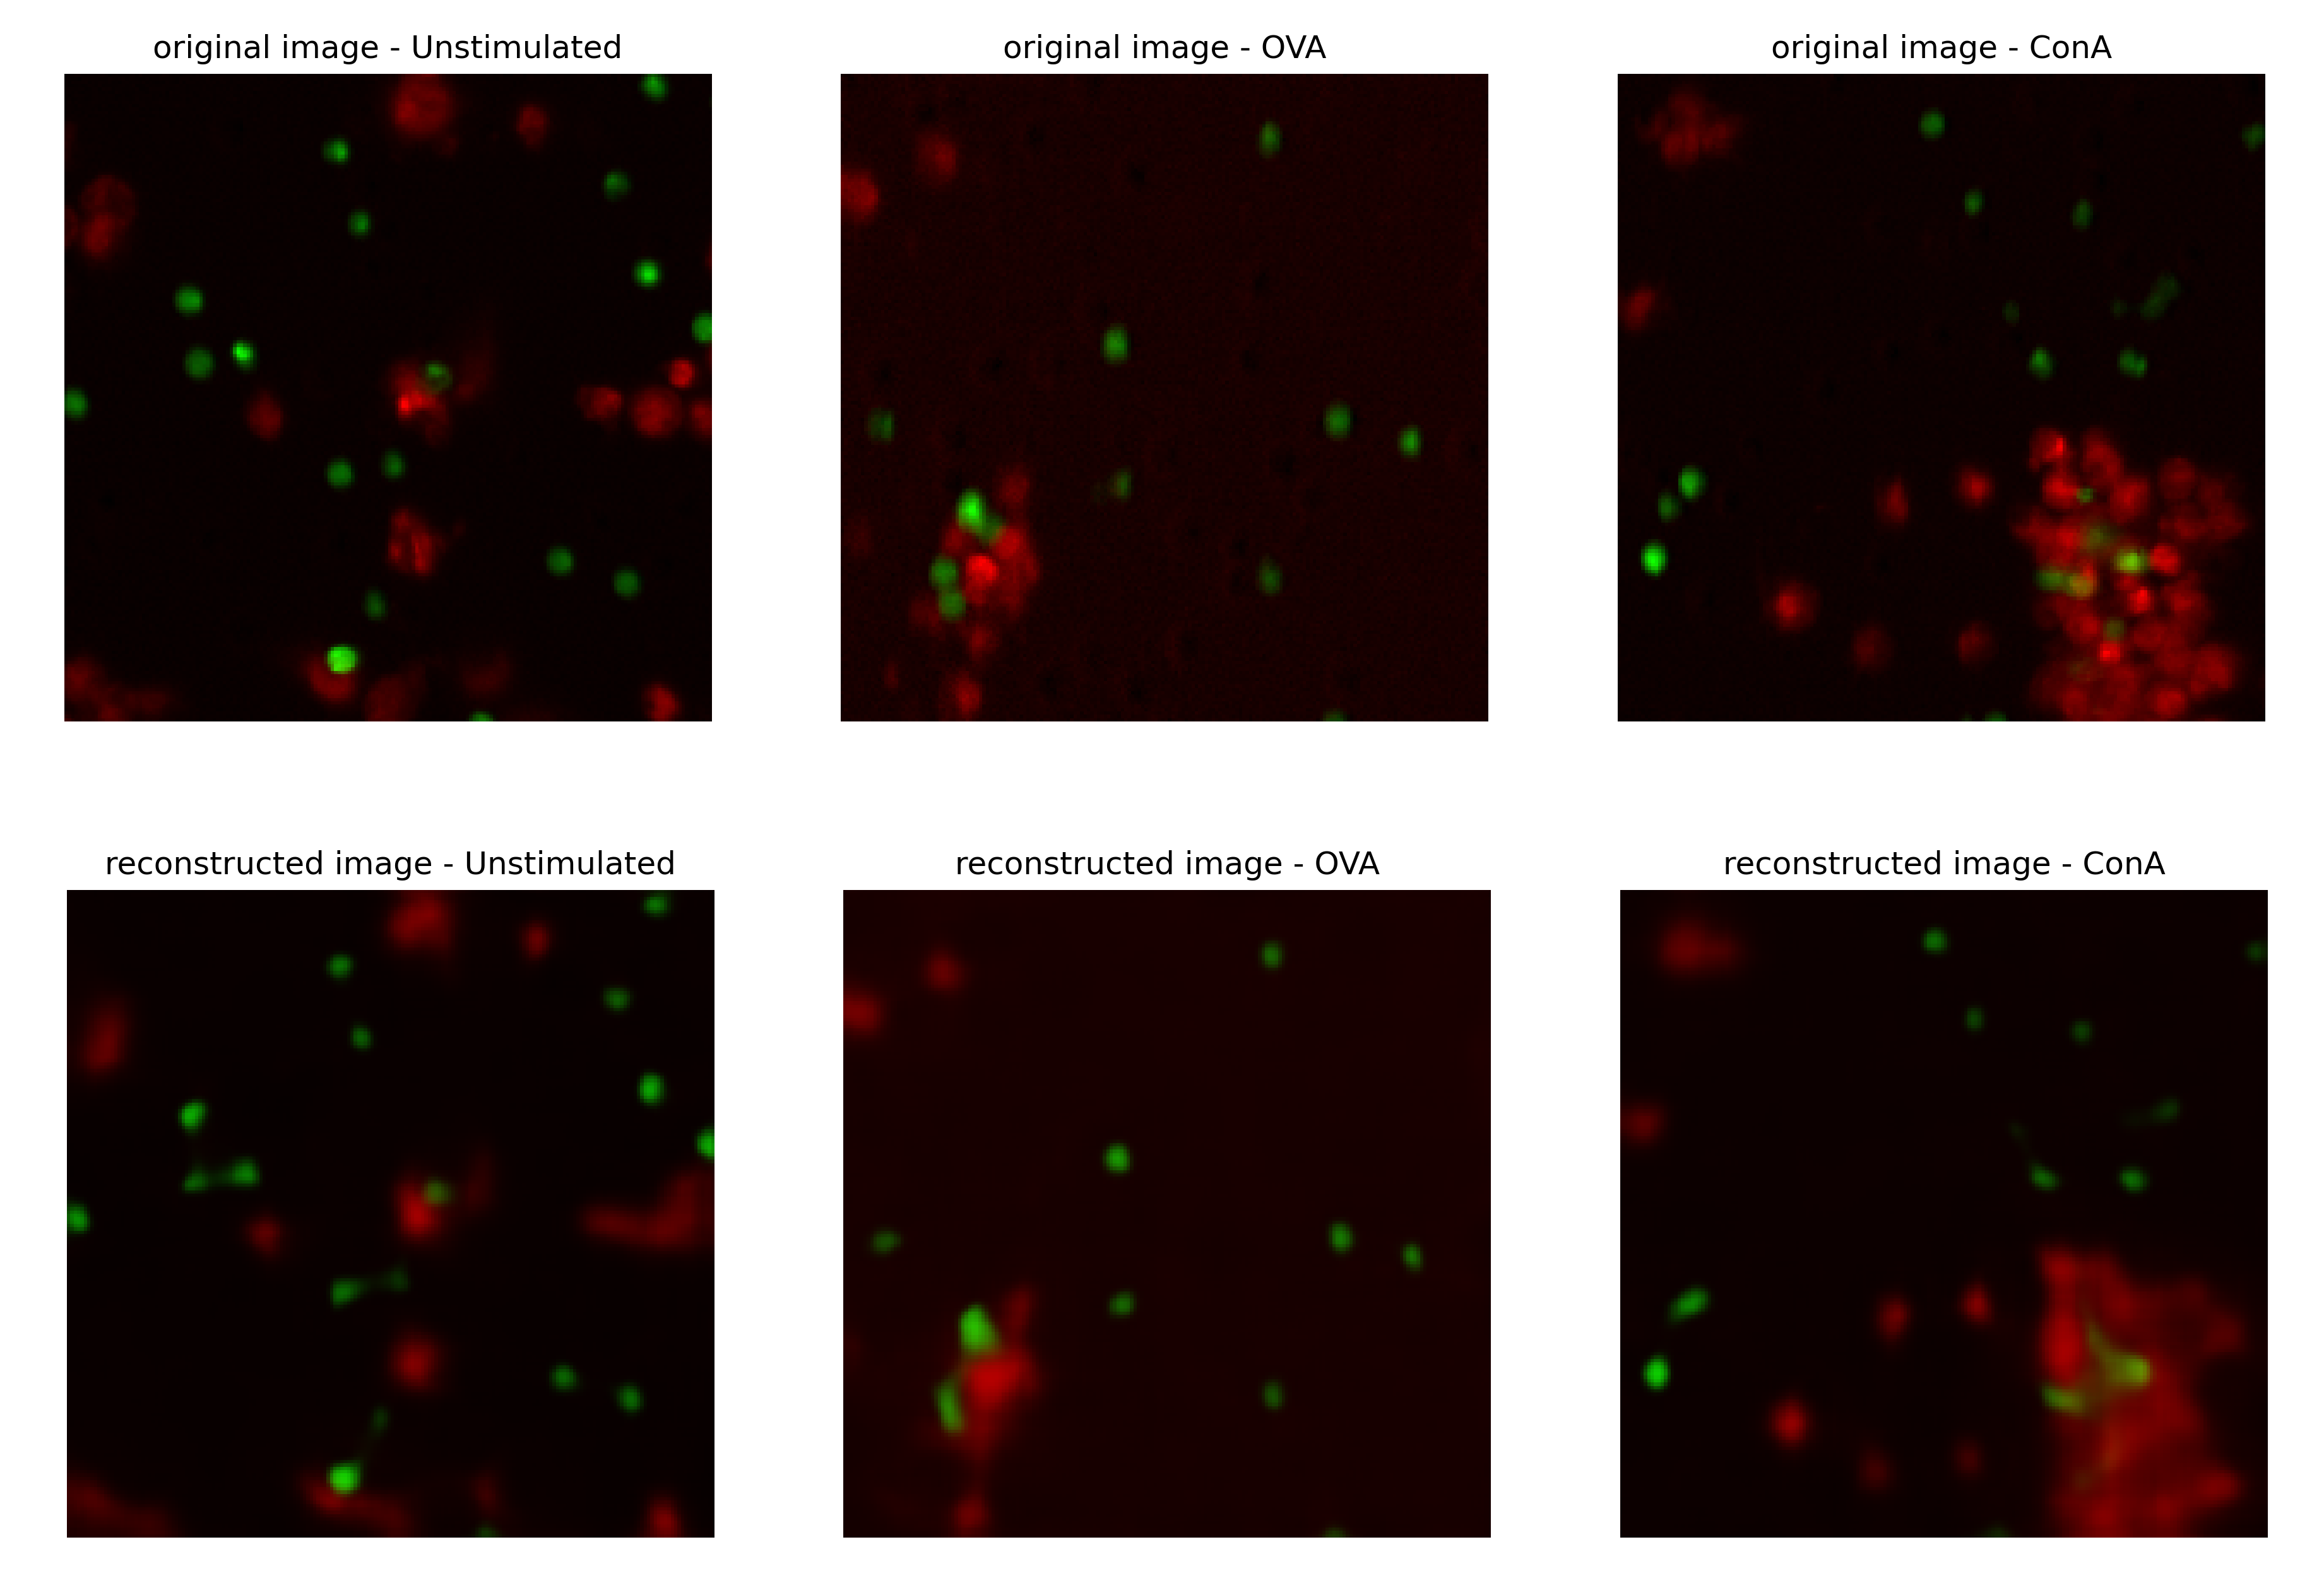
\includegraphics[width=\textwidth]{dissertation/figures/CK19_reconstruction.png}
        \caption{Normal images}
    \end{subfigure}
    \begin{subfigure}[h!]{0.45\textwidth}
        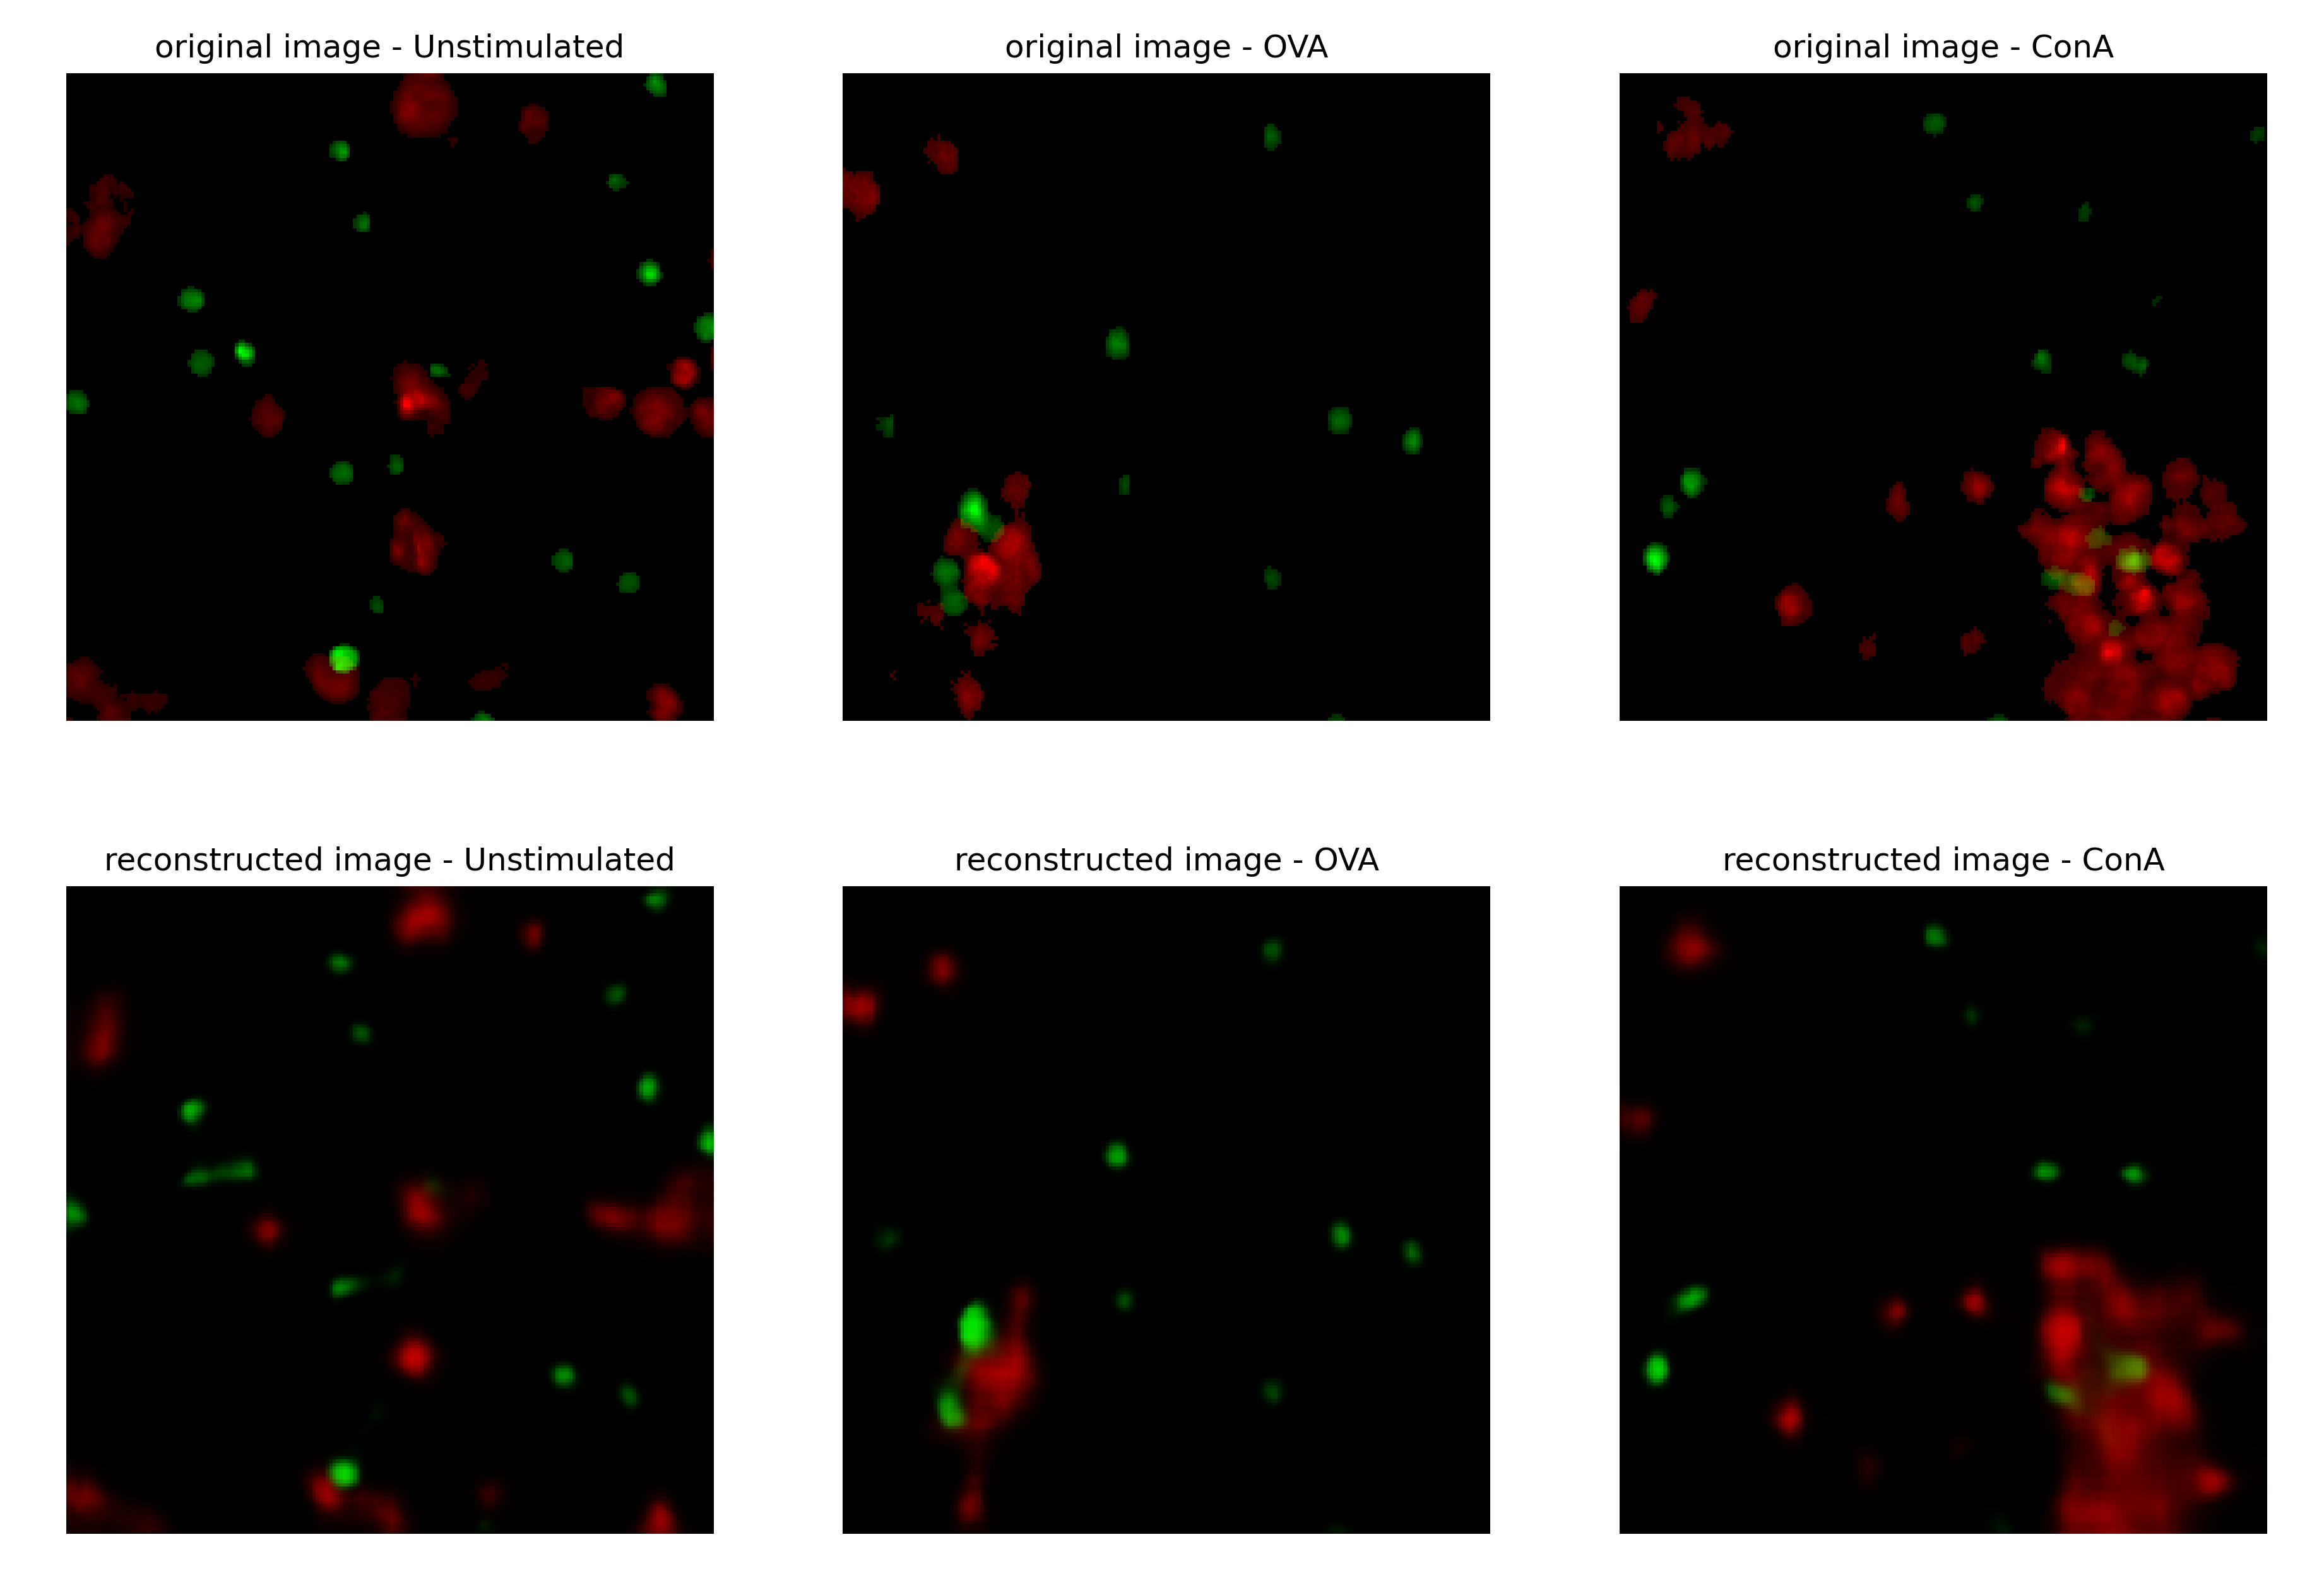
\includegraphics[width=\textwidth]{dissertation/figures/CK19_masked_reconstruction.png}
        \caption{Masked images}
    \end{subfigure}
    \caption{Autoencoder-reconstructed images from the full dataset. For each of the subfigures, categories are `Unstimulated', `OVA', `ConA' from left to right. Input images are at the top, and predicted images at the bottom.}
    \label{fig:my_label}
\end{figure}

\bigskip
\subsubsection{Dual dataset}
\hfill
\hfill

\begin{figure}[h!]
    \centering
    \begin{subfigure}[h!]{0.45\textwidth}
        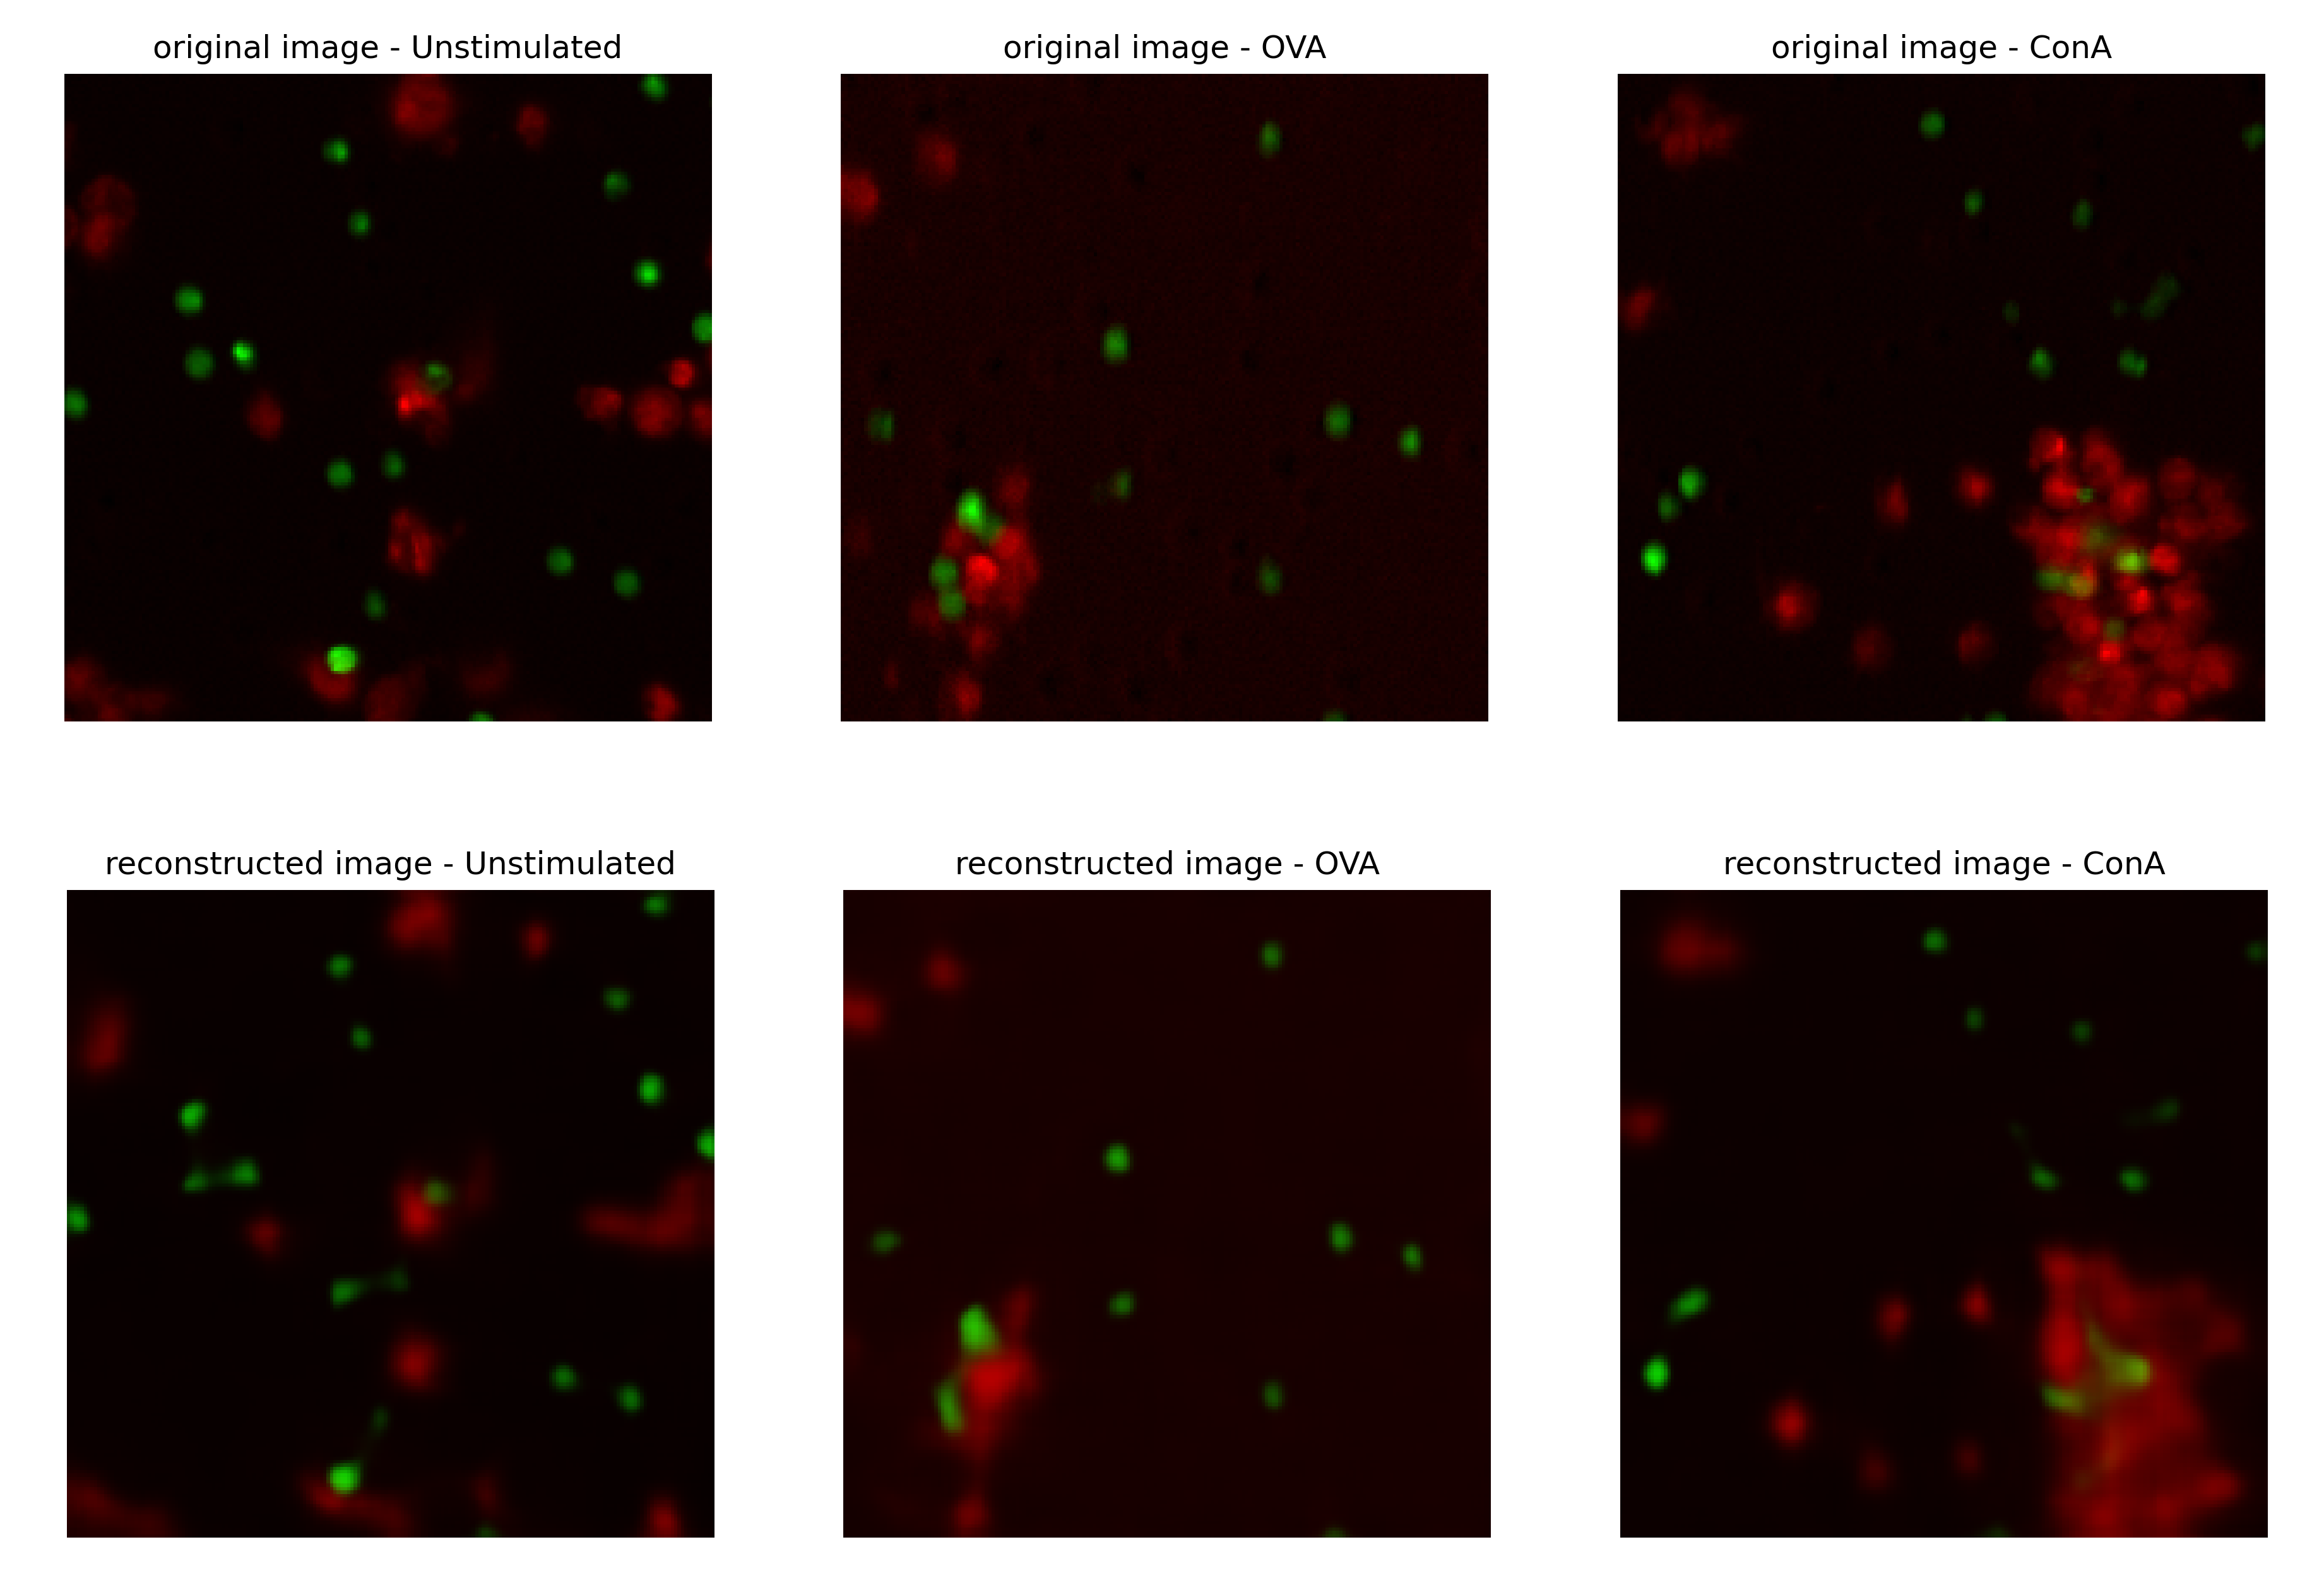
\includegraphics[width=\textwidth]{dissertation/figures/CK19_reconstruction.png}
        \caption{Normal images}
    \end{subfigure}
    \begin{subfigure}[h!]{0.45\textwidth}
        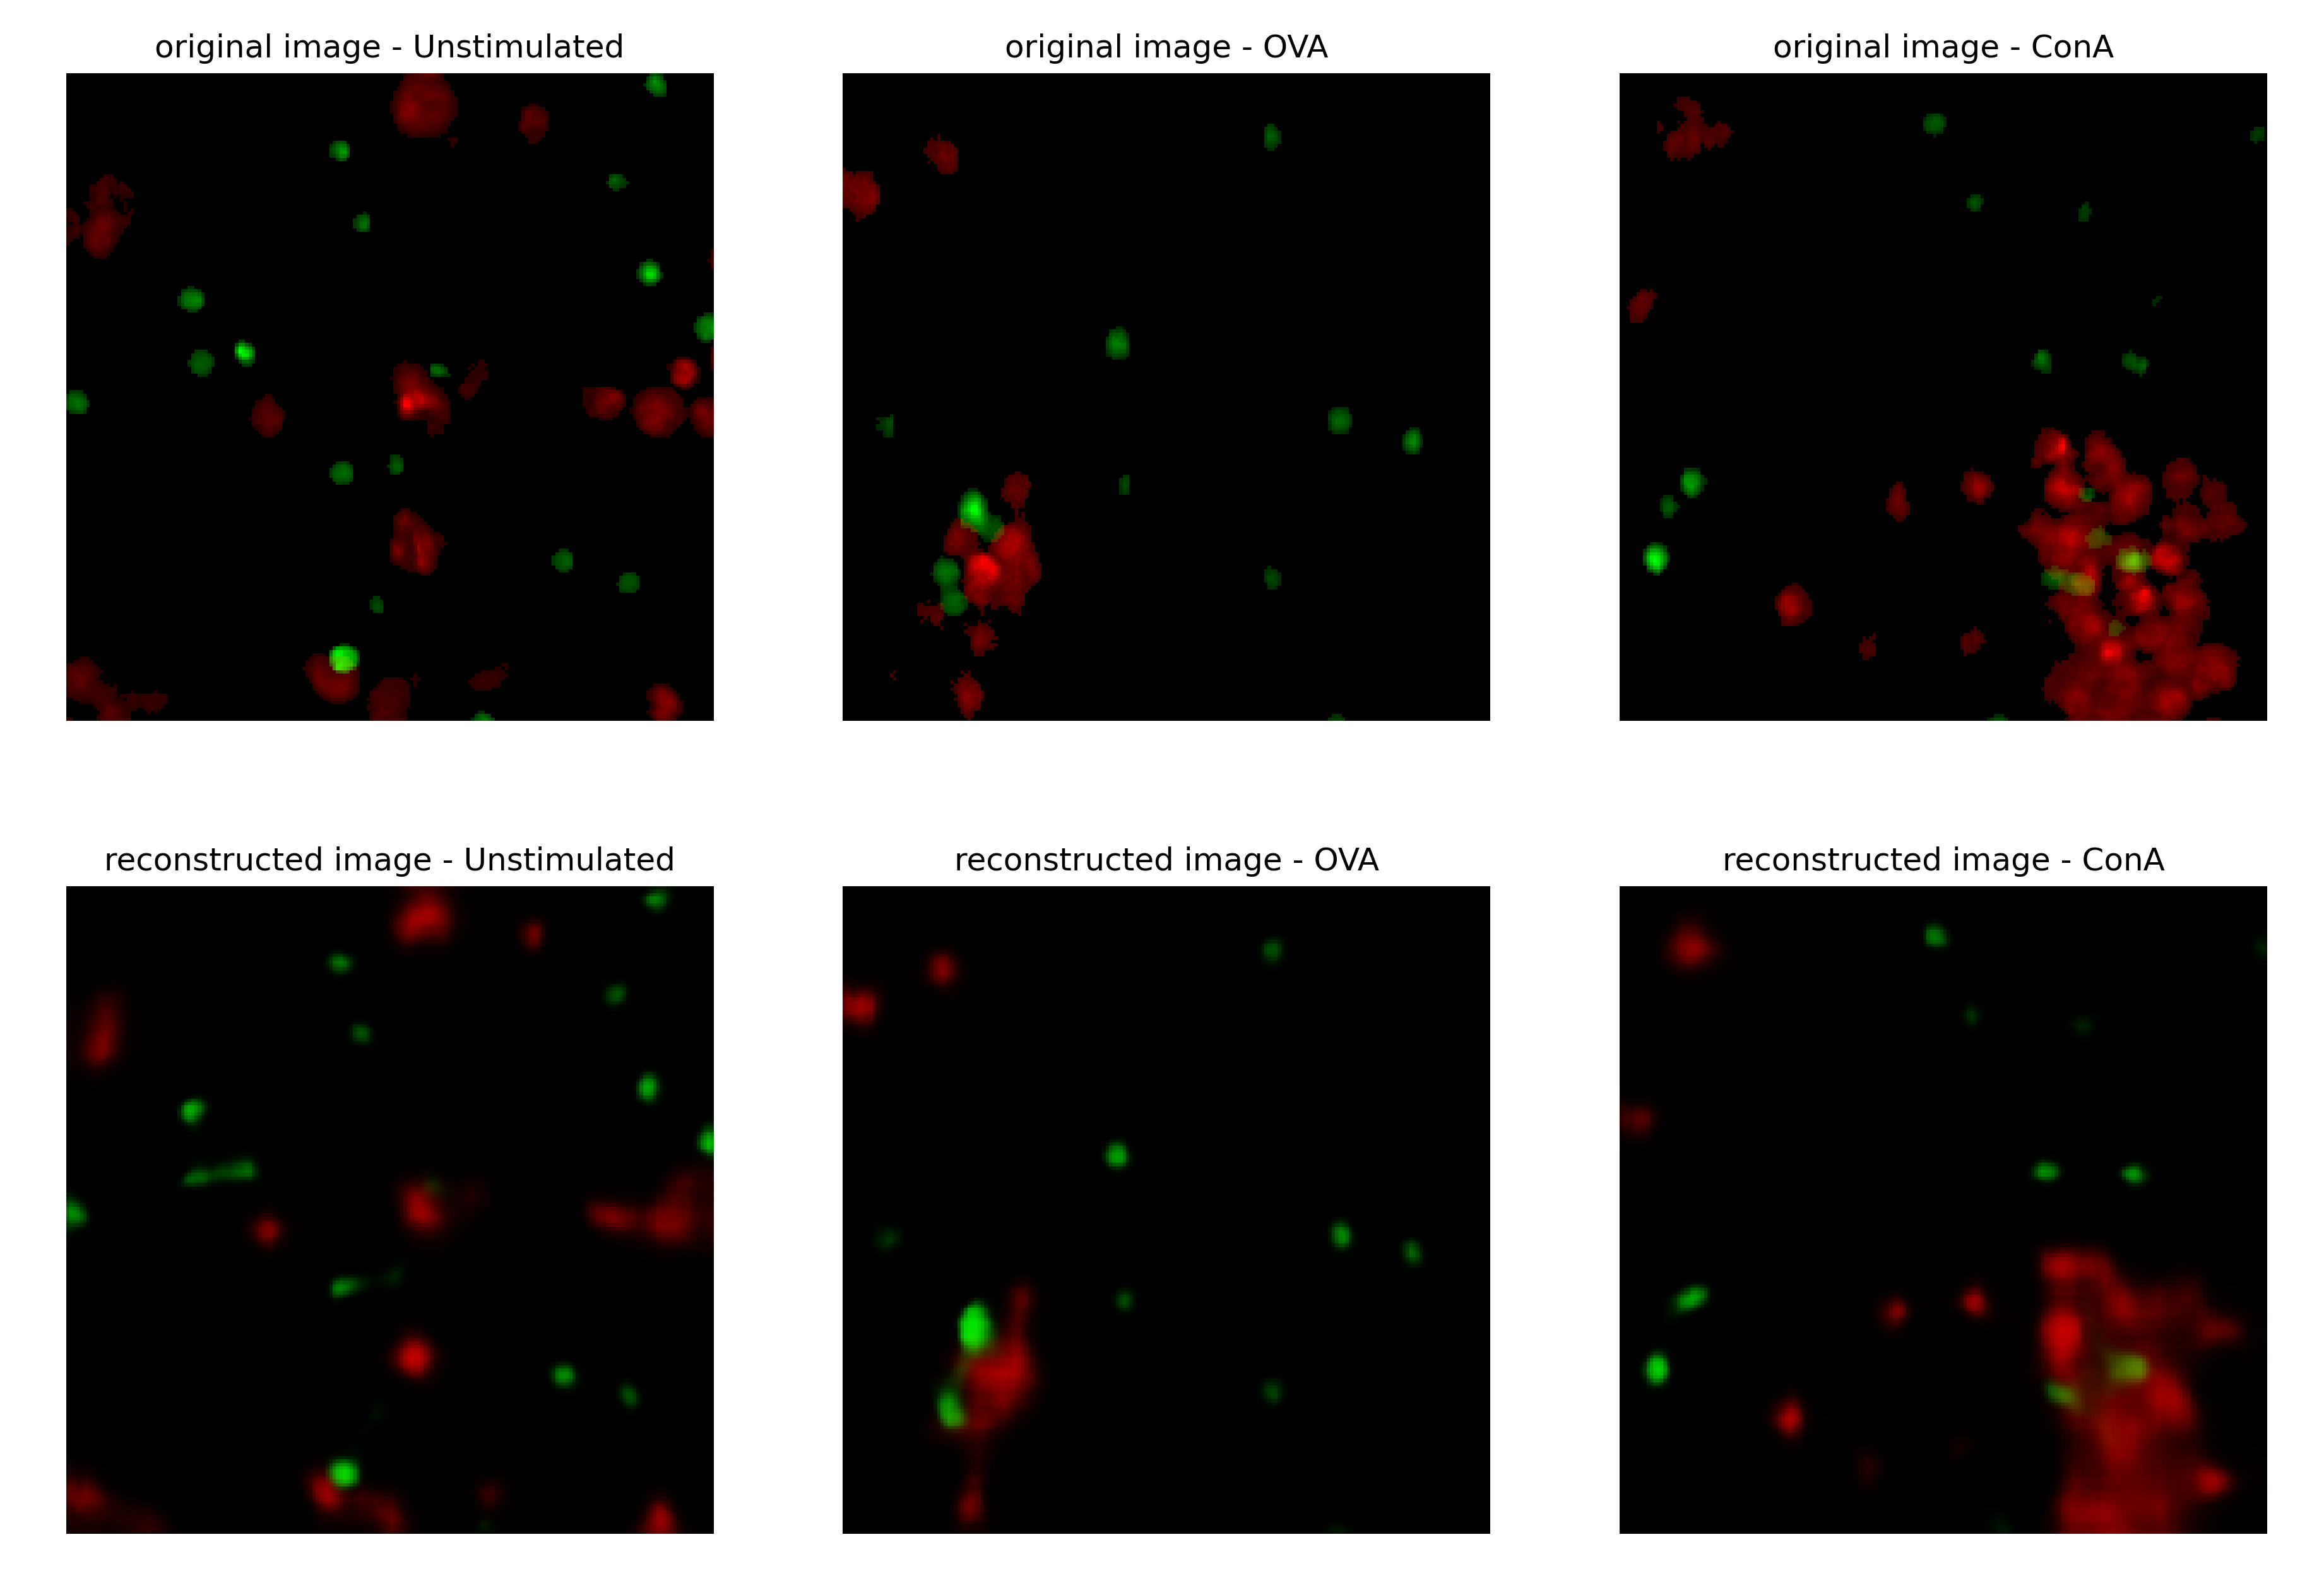
\includegraphics[width=\textwidth]{dissertation/figures/CK19_masked_reconstruction.png}
        \caption{Masked images}
    \end{subfigure}
    \caption{Autoencoder-reconstructed images from the full dataset. For each of the subfigures, categories are `Unstimulated', `OVA', `ConA' from left to right. Input images are at the top, and predicted images at the bottom.}
    \label{fig:my_label}
\end{figure}

\bigskip
\subsubsection{DMSO dataset}
\hfill
\hfill

\begin{figure}[h!]
    \centering
    \begin{subfigure}[h!]{0.45\textwidth}
        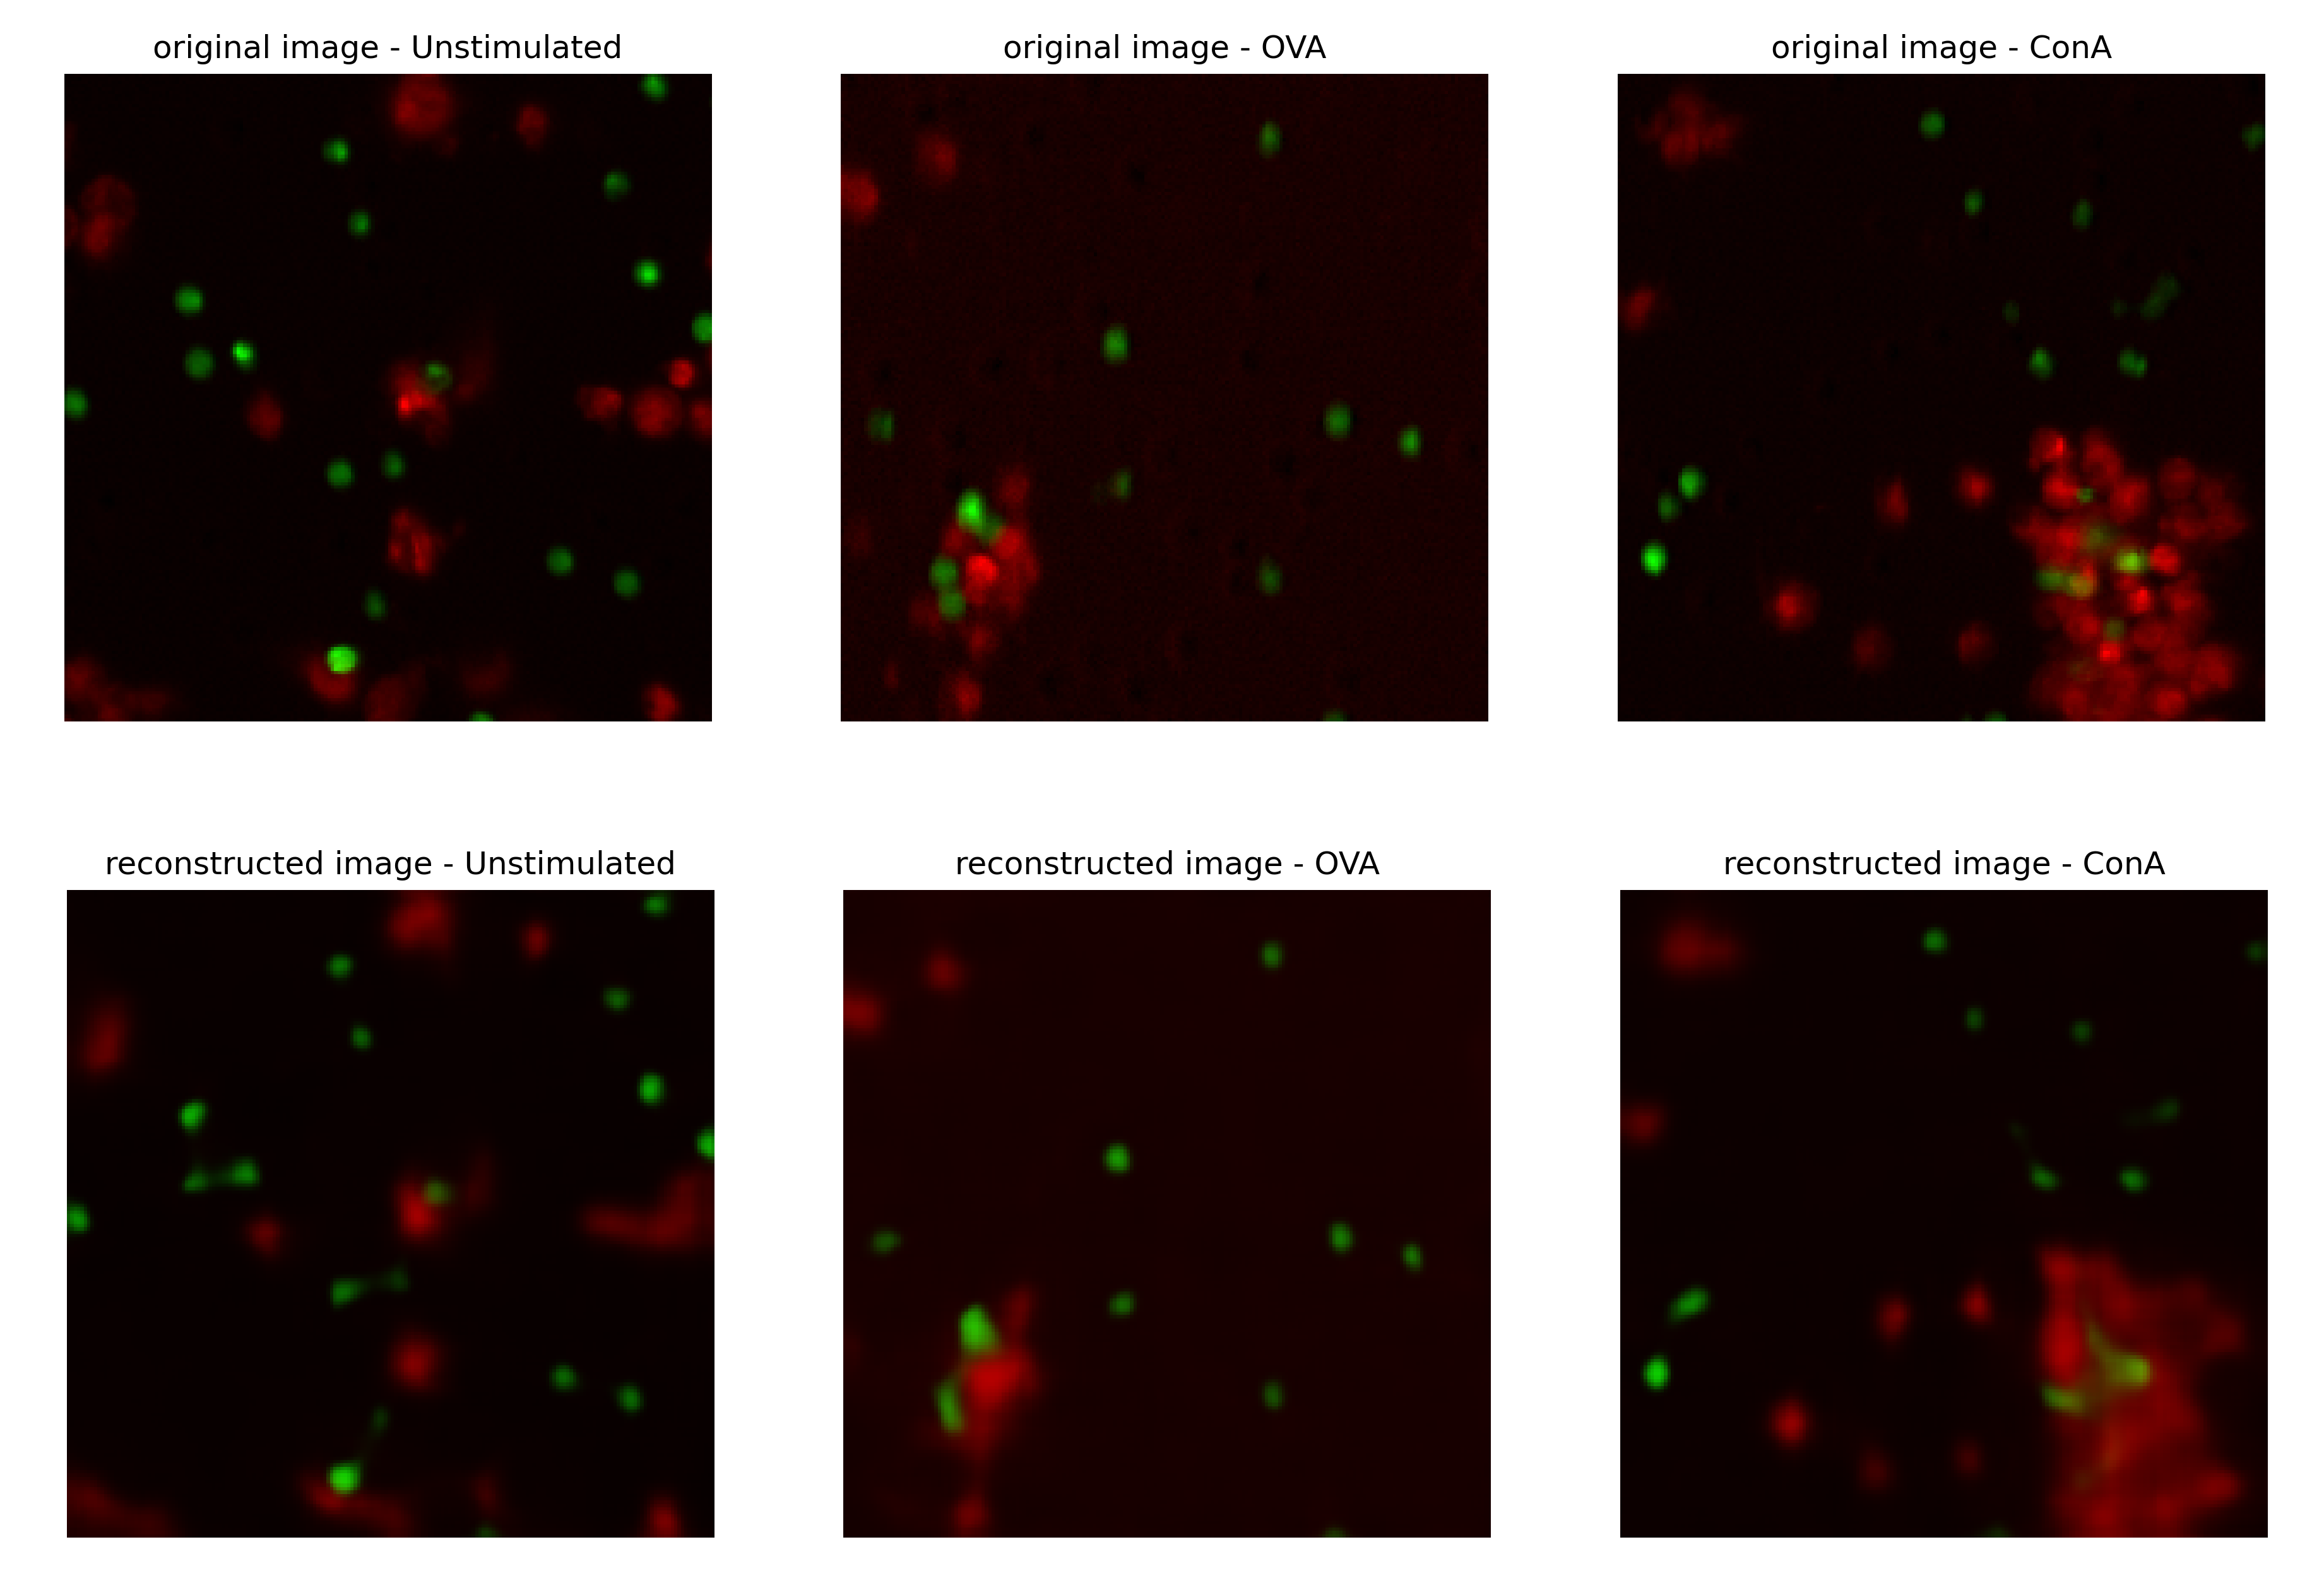
\includegraphics[width=\textwidth]{dissertation/figures/CK19_reconstruction.png}
        \caption{Normal images}
    \end{subfigure}
    \begin{subfigure}[h!]{0.45\textwidth}
        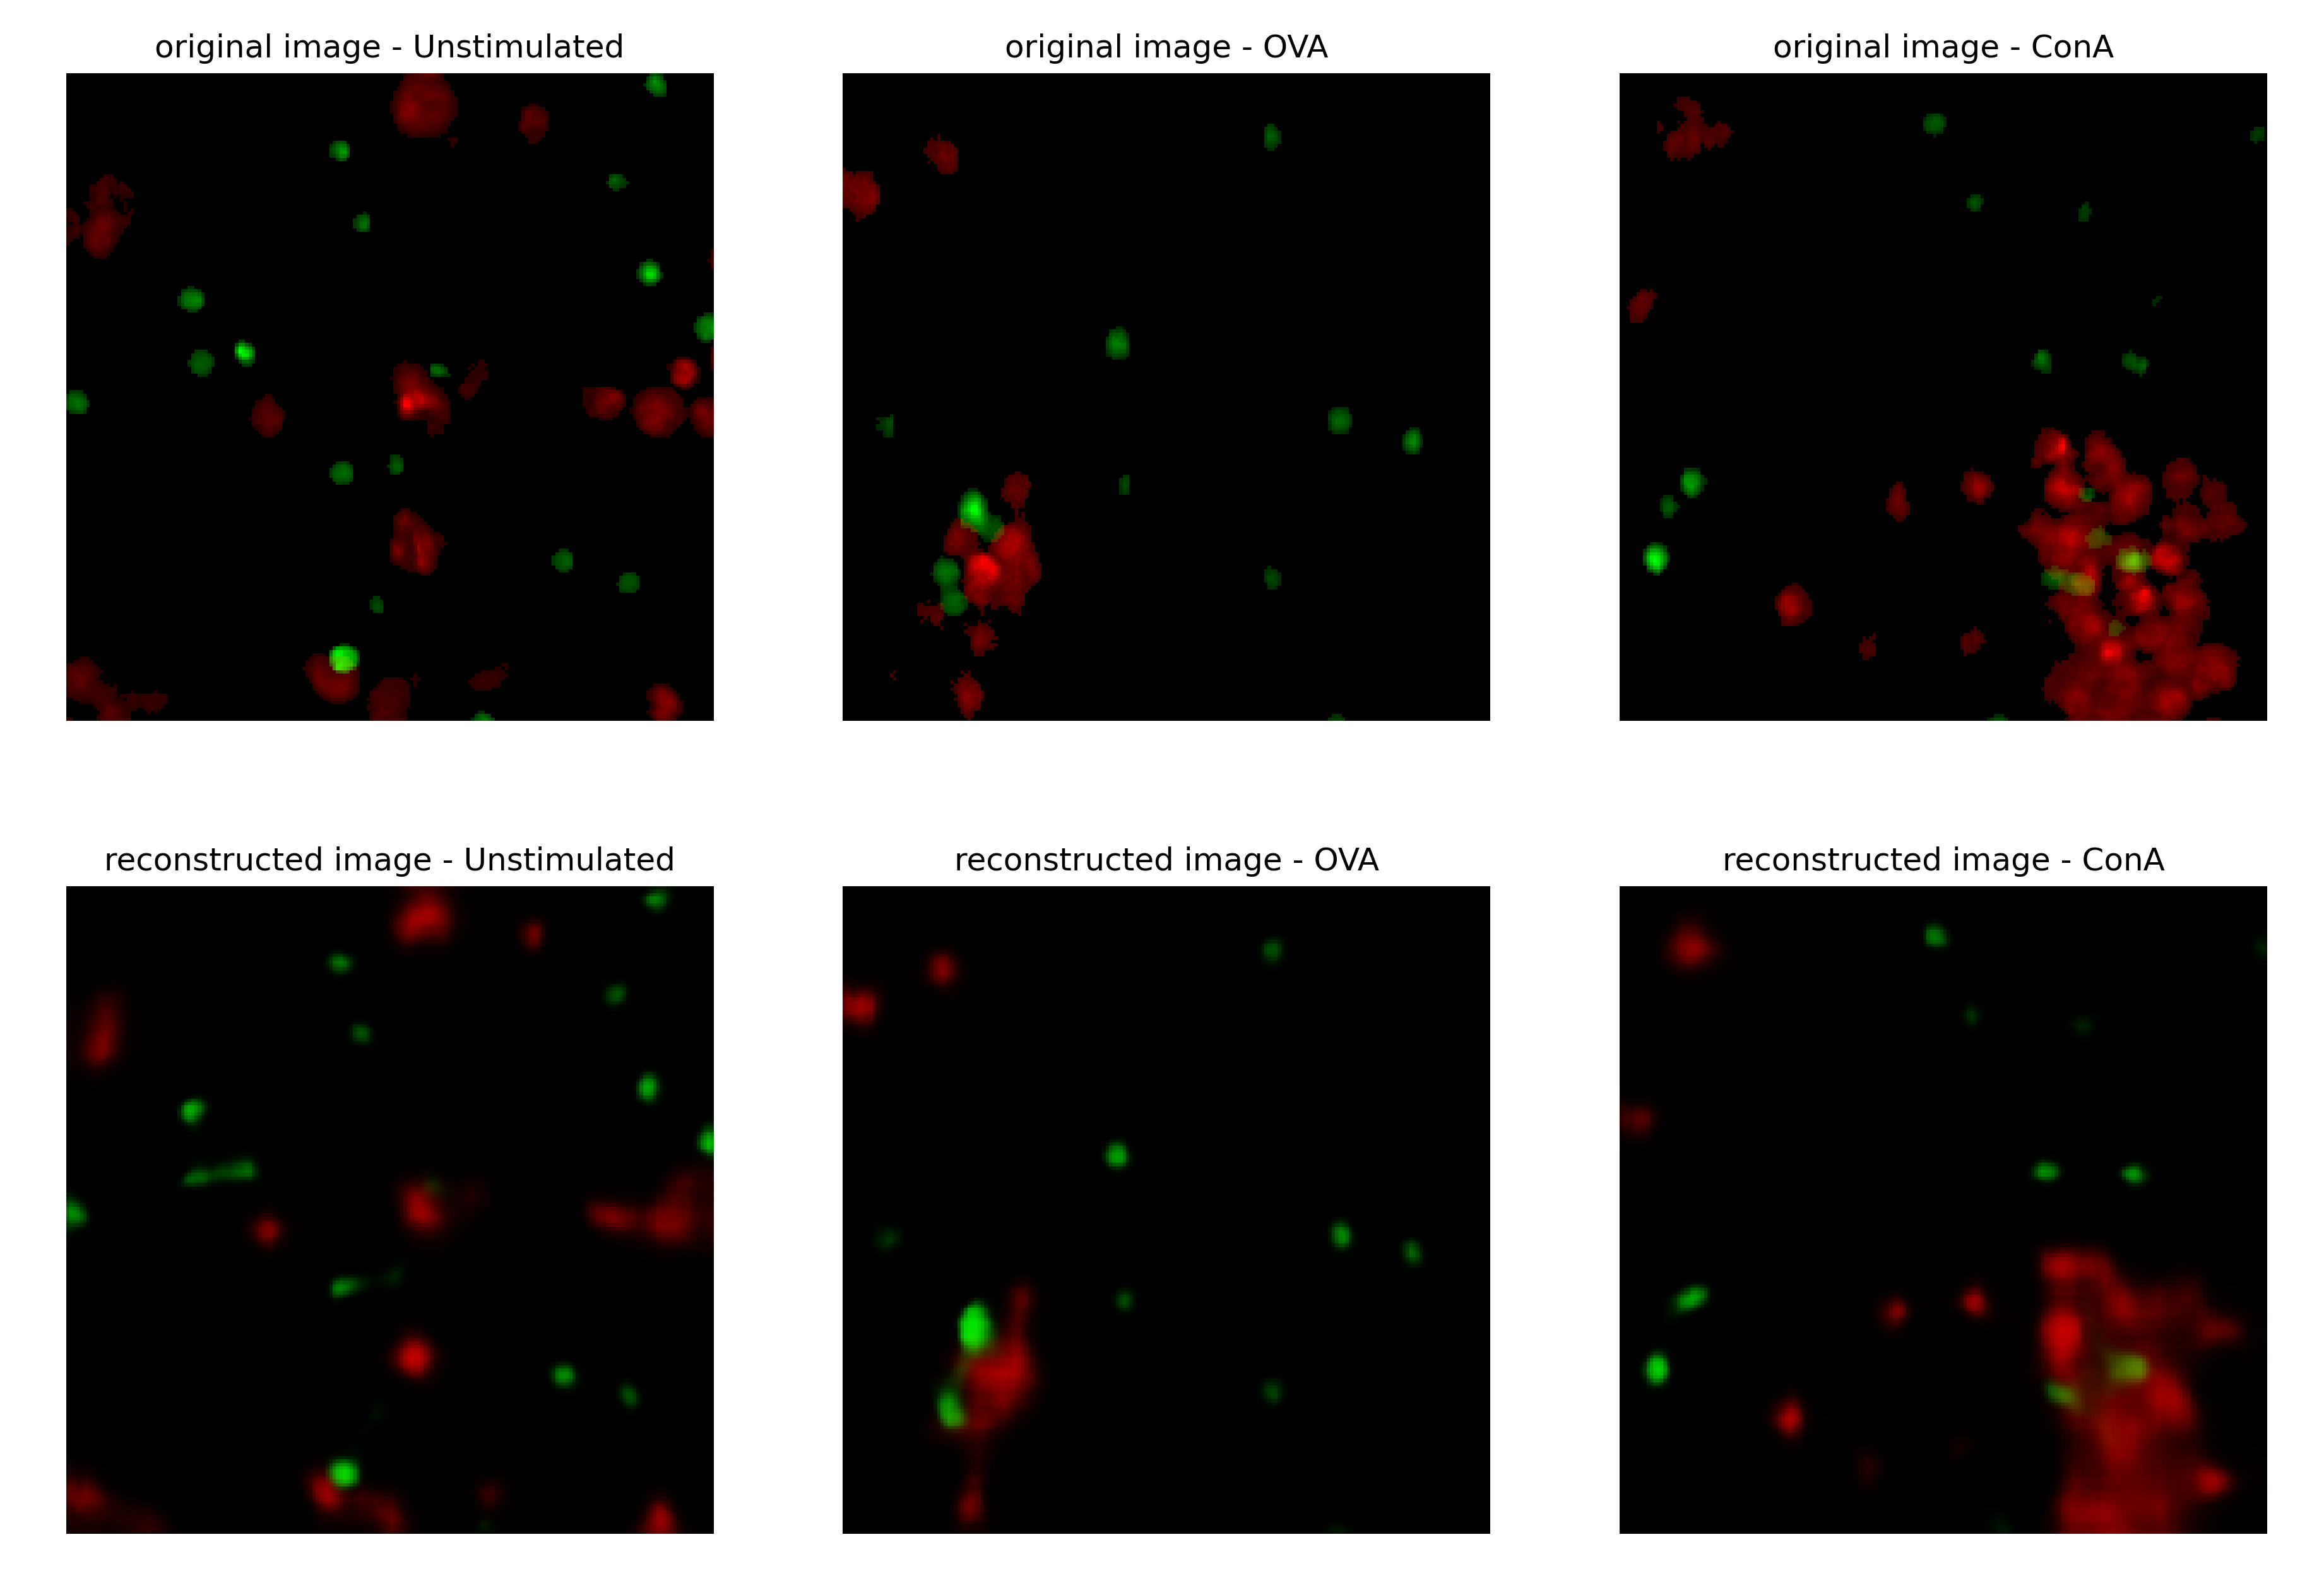
\includegraphics[width=\textwidth]{dissertation/figures/CK19_masked_reconstruction.png}
        \caption{Masked images}
    \end{subfigure}
    \caption{Autoencoder-reconstructed images from the full dataset. For each of the subfigures, categories are `Unstimulated', `OVA', `ConA' from left to right. Input images are at the top, and predicted images at the bottom.}
    \label{fig:my_label}
\end{figure}

The autoencoder received an input of 110,592 pixels. These pixels were reduced to a coded vector of 1,152. From this coded vector, we can see that the autoencoder reconstructed the images in quite a satisfactory way. Its main drawback is the way it merges different cells together.

\subsection{Can we find an underlying structure in the images of immune cells?}

The aim for two-dimensional visualisation of the datasets was that the visualisations would uncover clusters of images around the same experimental conditions.

\bigskip
\subsubsection{Baseline performance}
\hfill
\hfill

The expectations were that an autoencoder would allow us to extract the necessary features from an image that would be sufficient for it to be reconstructed, but also for it to be analysed. As such, we wanted to compare the visualisation performance of UMAP on the coded images to a baseline performance on raw images that have not been reduced in dimensionality. This was only ran for the full dataset as the large dimensions meant this computation took a considerable amount of time. On a 2015 MacBook Pro with i5 core and 8 GB of RAM, running UMAP on the 10,000 test instances of the full dataset of 110,592 pixel points each took 1 hour, 5 minutes and 33 seconds. The result visualisation is shown in Figure \ref{fig:baseline_vis}.

\begin{figure}[h!]
    \centering
    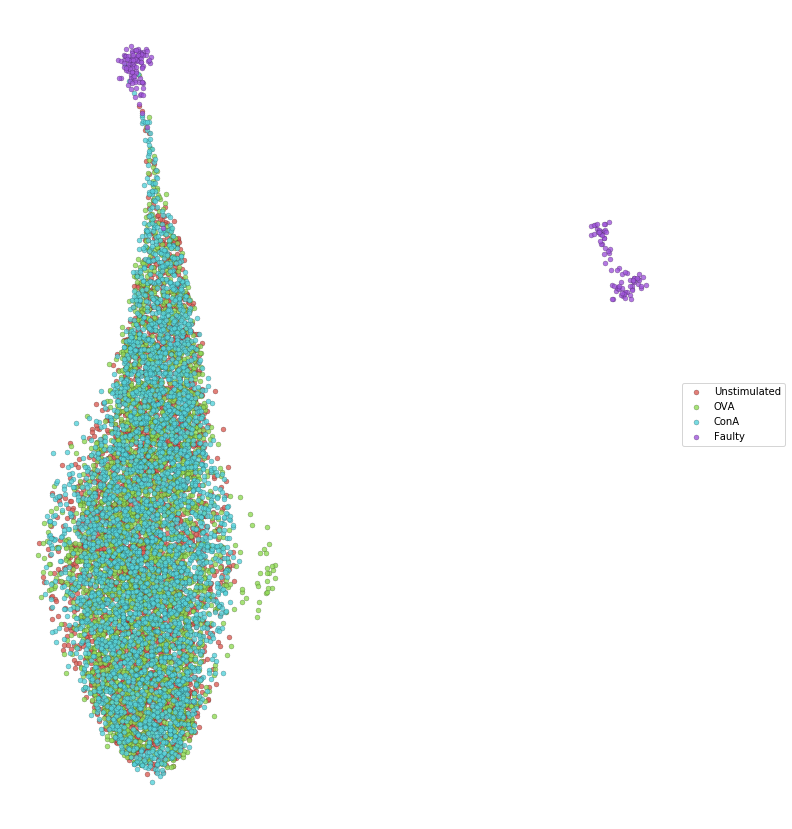
\includegraphics[width=0.45\textwidth]{dissertation/figures/CK19_baseline_visualisation.png}
    \caption{Two-dimensional UMAP projection of the 10,000 testing images in the full dataset. Each image counts 110,592 pixel points and is categorised into one of the `Unstimulated', `OVA', `ConA', or `Faulty' categories.}
    \label{fig:baseline_vis}
\end{figure}

This projection highlights that with the raw 192x193x3 images of immune cells, only `Faulty' images seem to be recognised and there is no clear distinction between images of other categories. We will now look whether reducing the dimensionality of the images with an autoencoder helps make this distinction.

\bigskip
\subsubsection{Full dataset}
\hfill
\hfill

\begin{figure}[h!]
    \centering
    \begin{subfigure}[h!]{0.45\textwidth}
        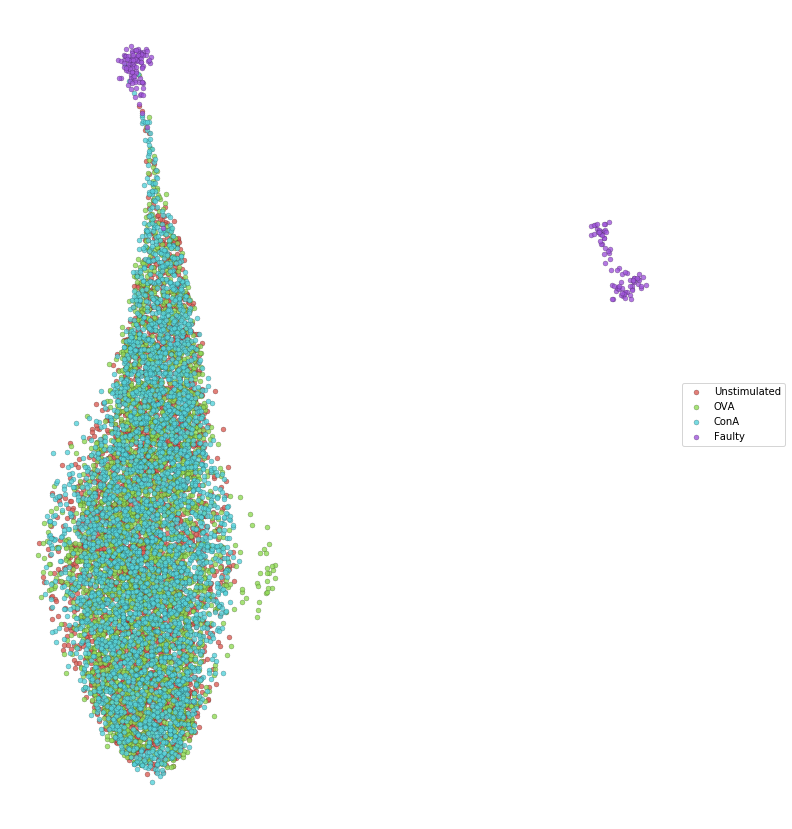
\includegraphics[width=\textwidth]{dissertation/figures/CK19_baseline_visualisation.png}
        \caption{Coded images}
    \end{subfigure}
    \begin{subfigure}[h!]{0.45\textwidth}
        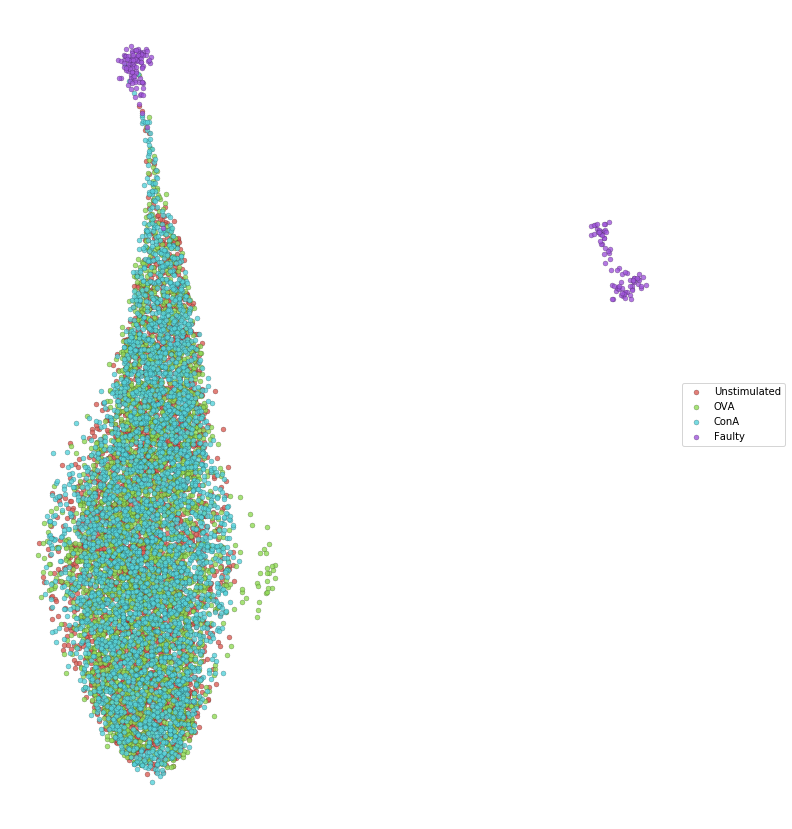
\includegraphics[width=\textwidth]{dissertation/figures/CK19_baseline_visualisation.png}
        \caption{Coded masked images}
    \end{subfigure}
    \caption{Two-dimensional UMAP projection of the 10,000 test images from the full dataset. Each image counts 1,152 pixel points and is categorised into one of the `Unstimulated', `OVA', `ConA', or `Faulty' categories.}
    \label{fig:my_label}
\end{figure}

This UMAP projection took [4 minutes] to run, which is a yx speed-up on the baseline performance. Moreover, we can see that some clusters have emerged.

\bigskip
\subsubsection{Dual dataset}
\hfill
\hfill

\begin{figure}[h!]
    \centering
    \begin{subfigure}[h!]{0.45\textwidth}
        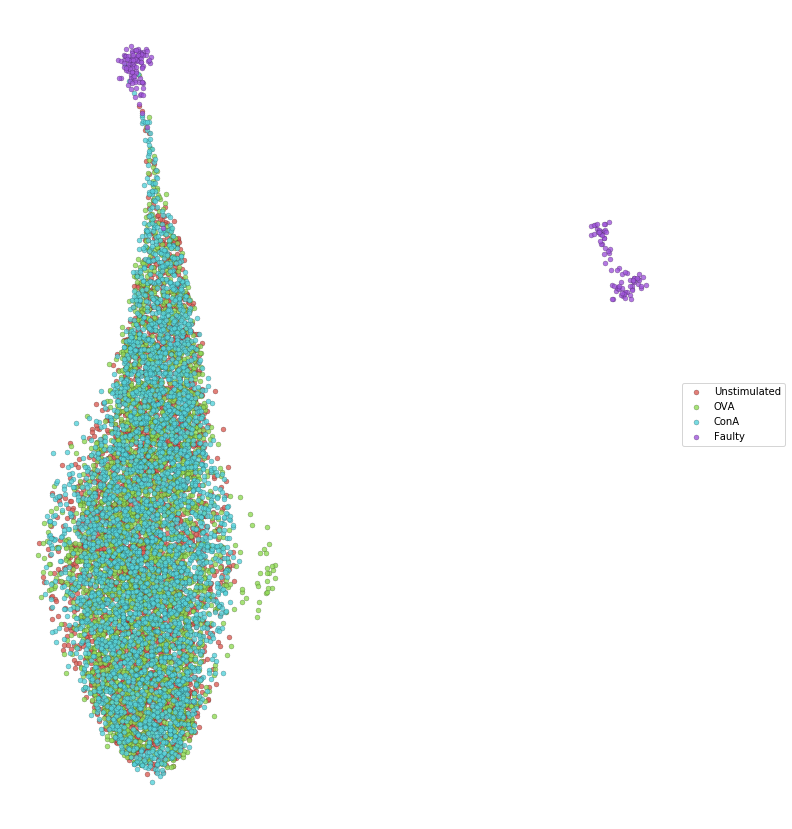
\includegraphics[width=\textwidth]{dissertation/figures/CK19_baseline_visualisation.png}
        \caption{Coded images}
    \end{subfigure}
    \begin{subfigure}[h!]{0.45\textwidth}
        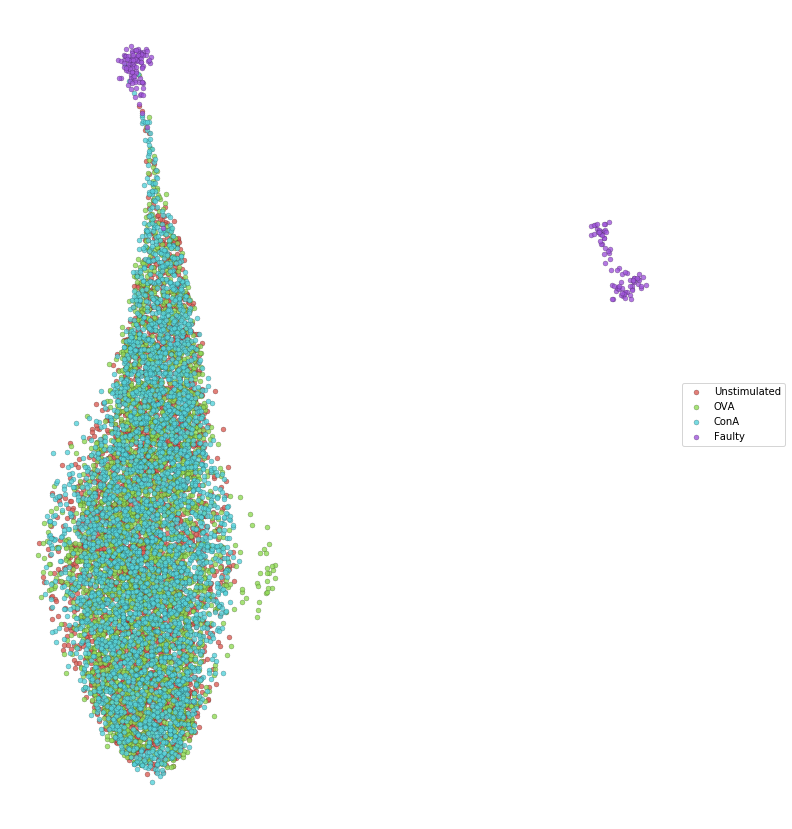
\includegraphics[width=\textwidth]{dissertation/figures/CK19_baseline_visualisation.png}
        \caption{Coded masked images}
    \end{subfigure}
    \caption{Two-dimensional UMAP projection of the 15,900 test images from the dual dataset. Each image counts 1,152 pixel points and is categorised into one of the `Unstimulated', `OVA', or `Faulty' categories.}
    \label{fig:my_label}
\end{figure}

\bigskip
\subsubsection{DMSO dataset}
\hfill
\hfill

\begin{figure}[h!]
    \centering
    \begin{subfigure}[h!]{0.45\textwidth}
        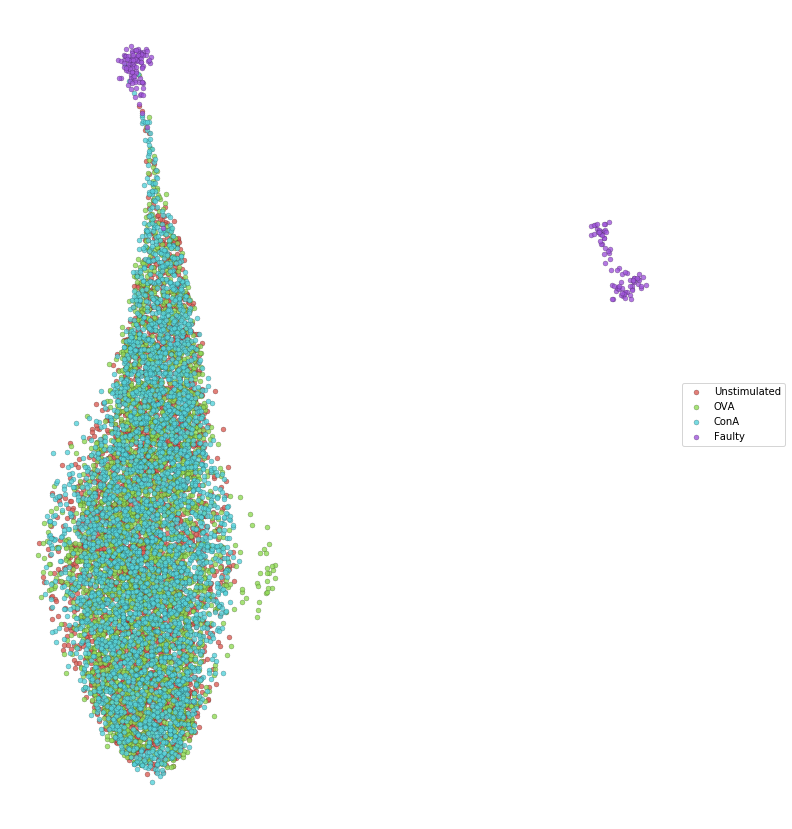
\includegraphics[width=\textwidth]{dissertation/figures/CK19_baseline_visualisation.png}
        \caption{Coded images}
    \end{subfigure}
    \begin{subfigure}[h!]{0.45\textwidth}
        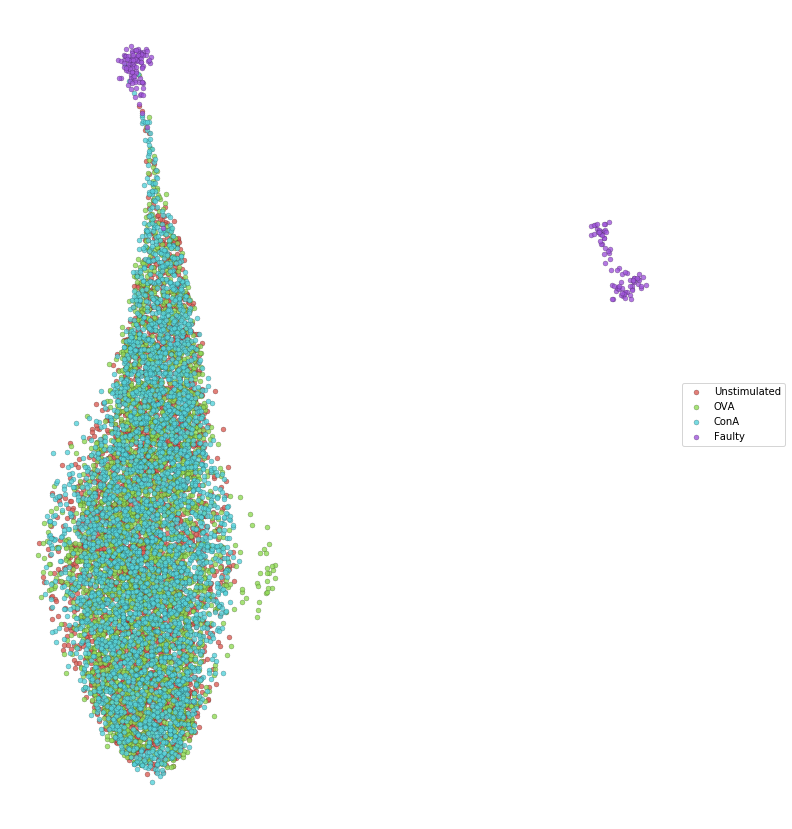
\includegraphics[width=\textwidth]{dissertation/figures/CK19_baseline_visualisation.png}
        \caption{Coded masked images}
    \end{subfigure}
    \caption{Two-dimensional UMAP projection of the 8,000 test images from the DMSO dataset. Each image counts 1,152 pixel points and is categorised into one of the `Unstimulated', `OVA', `ConA', or `Faulty' categories.}
    \label{fig:my_label}
\end{figure}

\bigskip
\subsubsection{Exploring outliers}
\hfill
\hfill

In order to explore the different clusters observed in the visualisations further, we developed a tool that makes use of matplotlib's animation API\footnote{https://matplotlib.org/api/animation\_api.html}. A user can hover over the points of the visualisation to display the image that was encoded and mapped to a point on the two-dimensional point. It is useful for looking at outlier points on the edges of clusters or in smaller clusters, but requires quite a lot of memory to update coordinates in a graph with a large number of points and display a 192x192x3 image, and is slow in such cases.

Figures \ref{} highlight the tool's functionality.

\subsection{Are our visualisations more meaningful with interaction measure meta-data?}

Although UMAP supports supervised dimensionality reduction, all our computations were ran unsupervised. We did not feed any labels into the algorithm, and they were only added to the visualisation later on. As such, in the case of visualisations that did yield some groupings, but contained points of mixed categories, we hypothesised that other meta-data about the images might explain why some clusters were formed. Indeed, maybe the between-differences of images in different categories were not strong enough, but the algorithm would be able to split the images on the basis of something else, for example, how much the cells overlapped in the image, regardless of their stimulation category.

We plotted the visualisations again, but using the interaction measures collected with the intersection-over-union metric to change the size of the markers. We decided to tweak the visualisations shown in Figure \ref{}, etc. as they yielded some interesting clusters. The results are shown in Figure \ref{} below.

From this we can see that there is some meaningful structure to the data that the autoencoder was able to uncover, however, the groupings obtained are not specific to stimulation categories, but the amount of interaction per image.

\section{Regression}

Our regression task is to predict the percentage of overlap between T-cells and dendritic cells from an image where T-cells are shaded green, and dendritic cells are shaded red.

\subsection{Regression metrics}

Our regression model is trained on mean squared error (MSE) and we decided to evaluate on root-mean-square-error (RMSE) as it is a common metric for evaluating the difference between predictions of a model and actual truth values. RMSE has the advantage of being in the same unit as the dependent variable, which in our case is the percentage of overlap between the cells objects obtained with intersection-over-union. RMSE is defined as the square root of the quadratic mean of the difference between our predicted values and their truth values. The equation is as follows:

\begin{equation*}
    RMSE = \sqrt{\frac{1}{n}{\Sigma_{i=1}^{n}{\Big({\hat{y}_i-y_i})}^2}}
\end{equation*}

where $n$ is the number of samples in the dataset, $y$ is the true value of a sample, and $\hat{y}$ is the predicted value of a sample.

We also include the (unbiased) standard deviation (SD) of our predicted results to express their variability. The formula for SD is as follows:

\begin{equation*}
    \sigma = \sqrt{\frac{1}{n-1}\Sigma_{i=1}^{n}{(\hat{y}_i - \mu)}^2}
\end{equation*}

where $n$ is the number of predicted samples, $\hat{y}_i$ is the predicted value of a sample and $\mu$ is the mean of all predicted values.

\subsection{Can we quantify interaction from an image of immune cells?}

\section{Discussion}

As we can see there does not seem to be an underlying structure to the data that is dependent on stimulation levels. This might be because of the window size.
